\documentclass[]{cv-class}
\usepackage{afterpage}
\usepackage{hyperref}
\usepackage{color}
\usepackage{xcolor}
\usepackage[document]{ragged2e}

\hypersetup{
    colorlinks=true,
    linkcolor=blue
}

\RequirePackage{xcolor}
\definecolor{pblue}{HTML}{0395DE}

\begin{document}
\header{Carlos Eduardo}{Orozco}
{Analista/Dev Java Senior - Arquitecto de soluciones }

\vspace{1.15cm}
\fcolorbox{white}{gray}{\parbox{\dimexpr\textwidth-2\fboxsep-2\fboxrule}{%
	.....
}}

\begin{aside}
	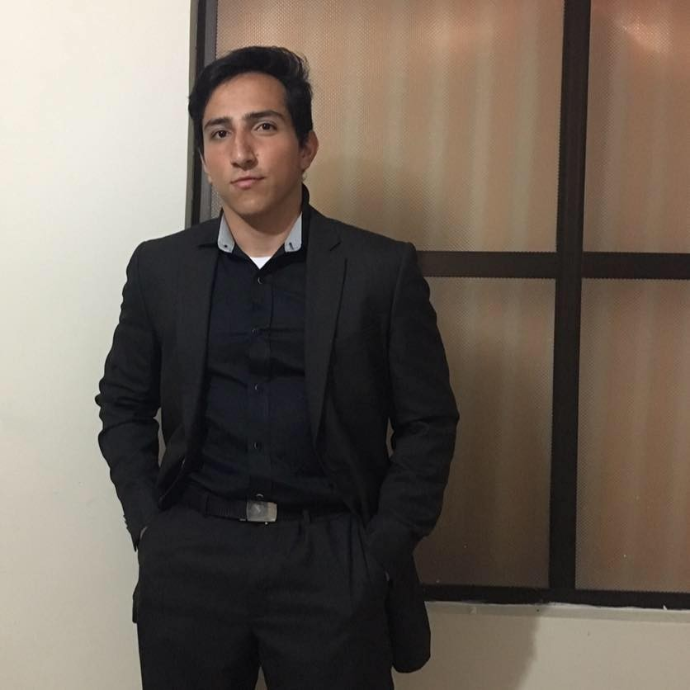
\includegraphics[scale=0.15]{img/indice.png}
	~
	\vspace{0.35cm}
	\section{Info/Contacto}
	\textbf{Edad:} 26 \\
	\textbf{Estado civil:} Soltero \\
	\textbf{Direccion:} Cra 51D 67A16 \\
	\textbf{Ciudad:} Medellín, CO \\ 
	\textbf{Contacto/Correo:}\\ \href{https://api.whatsapp.com/send?phone=573116345180}{\raisebox{-0.35ex}{
\includegraphics[scale=0.06]{img/whatsapp-logo.jpg}}/+573116345180}\\
	\href{https://join.skype.com/invite/GVNxPbWtJxdc}{\raisebox{-0.35ex}{
\includegraphics[scale=0.1]{img/skype-logo.png}}/carlos.orozco22}\\
	\href{mailto:carlos940807@gmail.com}{\raisebox{-0.35ex}{
\includegraphics[scale=0.009]{img/gmail-logo.png}}/carlos940807}
	~
	\section{Info/Trabajo}
	\href{https://linkedin.com/in/corozco9408}{\raisebox{-0.35ex}{
\includegraphics[scale=0.3]{img/linkedin-logo.png}}/corozco9408}\\
	\href{https://www.researchgate.net/profile/Carlos_Orozco29}{\raisebox{-0.35ex}{
\includegraphics[scale=0.05]{img/researchgate-logo.png}}/carlos.orozco29}\\  	\href{https://orcid.org/0000-0003-2615-3294}{\raisebox{-0.35ex}{
\includegraphics[scale=0.7]{img/orcid-logo.png}}/0000-0003-2615-3294}
	~ 
	\section{Info/Académico}
	{\raisebox{-0.35ex}{
\includegraphics[scale=0.05]{img/unicauca-logo.png}}} \textbf{Universidad del Cauca} \\
	\href{mailto:carlosorozco@unicauca.edu.co}{carlosorozco@unicauca.edu.co}
	{\raisebox{-0.35ex}{
\includegraphics[scale=0.05]{img/udea-logo.png}}}\textbf{Universidad de Antioquia} \\
	\href{mailto:carlose.orozco@udea.edu.co}{carlose.orozco@udea.edu.co}

	~
	\section{Lenguas}
	\asidelist{\textbf{Español}}
	{
\includegraphics[scale=0.40]{img/5stars.png}}
	\asidelist{\textbf{Inglés}}
	{
\includegraphics[scale=0.40]{img/4stars.png}}
	~

	\section{FrontEnd}
	\asidelist{\textbf{Angular 4+}}
	{
\includegraphics[scale=0.40]{img/5stars.png}}
	\asidelist{\textbf{Ionic}}
	{
\includegraphics[scale=0.40]{img/5stars.png}}
	~

	\section{BackEnd}
	\asidelist{\textbf{Java EE}}
	{
\includegraphics[scale=0.40]{img/5stars.png}}
	\asidelist{\textbf{Python 3.x}}
	{
\includegraphics[scale=0.40]{img/5stars.png}}
	\asidelist{\textbf{C\#}}
	{
\includegraphics[scale=0.40]{img/4stars.png}}
	\asidelist{\textbf{REST/SOAP}}
	{
\includegraphics[scale=0.40]{img/5stars.png}}
	~

	\section{Bases de datos}
	\asidelist{\textbf{Oracle}}
	{
\includegraphics[scale=0.40]{img/5stars.png}}
	\asidelist{\textbf{MySql}}
	{
\includegraphics[scale=0.40]{img/5stars.png}}
	\asidelist{\textbf{PostgreSql}}
	{
\includegraphics[scale=0.40]{img/5stars.png}}

\end{aside}

\justifying
	\begin{small}
\textit{
    Soy un ingeniero de sistemas con experiencia en desarrollo BackEnd. Mis habilidades principales se enfocan al análisis y desarrollo en áreas de la salud y el sector financiero. Actualmente trabajo como arquitecto/desarrollador java senior y consultor de procesos de GCS. Adicionalmente, realizo trabajo de investigación activa en las áreas de la GCS, mejora de procesos, DevOps, mejores prácticas en arquitectura y aseguramiento de la calidad.}
	\end{small}

\section{Experiencia}
\begin{entrylist}
	\entry
	{Dic. 19 - Hoy}
	{Arquitecto de soluciones}
	{DAWSIN SAS, Popayán, CO}
	{Llevar a cabo la validación y monitoreo de la arquitectura de nuevas soluciones desarrolladas por la organización para asegurar su integridad y escalabilidad con el paso del tiempo.}

	\entry
	{Mar. 17 - Hoy}
	{Consultor independiente}
	{Medellín and Popayán, CO}
	{Realizar consultoría en temas relacionados a mejores prácticas de desarrollo y arquitectura de soluciones informáticas de acuerdo a su arquitectura, mejora de procesos y aseguramiento de la calidad.}
	  
	\entry
	{Oct. 19 - Hoy}
	{Desarrollador Senior}
	{ \raisebox{-1.5ex}{
\includegraphics[scale=0.04]{img/tecso-logo.jpg}Tecso Ltda, Medellín, CO}}
	{Llevar a cabo la implementación de asignaciones relacionadas al BackEnd de soluciones para clientes específicos en el sector financiero (implementación de servicios web, base de datos, definición de rutas y canales de comunicación, desarrollo de nuevos requerimientos y validación de nuevas iniciativas)}
	\entry
	{Nov. 18 - Oct. 19}
	{Arquitecto de software}
	{ \raisebox{-1.5ex}{
\includegraphics[scale=0.09]{img/sew-logo.jpg}Servicios en Web, Medellín, CO}}
	{Realizar la definición, planeación, desarrollo y análisis técnico y funcional de los productos desarrollados por la empresa para asegurar que cumplen estándares de calidad y buenas prácticas durante el ciclo de vida del producto y el desarrollo.}
	    
	\entry
	{Aug. 18 - Nov. 18}
	{Analista/Desarrollador}
	{ \raisebox{-1.5ex}{
\includegraphics[scale=0.09]{img/sew-logo.jpg}Servicios en Web, Medellín, CO}}
	{Realizar tareas de análisis, desarrollo e implementación de soluciones basadas en productos relacionados al comercio electrónico.}
	
	\entry
	{Jul. 16 - Jul. 18}
	{Desarrollador FullStack}
	{ \raisebox{-1.5ex}{
\includegraphics[scale=0.05]{img/sitis-logo.png} SITIS SAS, Popayán, CO}}
	{Desarrollo de soluciones para la organización usando tecnologías específicas (JAVA EE, Primefaces, Angular 6x, JPA, Hibernate, Oracle DB)}
	
	\entry
	{Mar. 13 - Abr 15}
	{Desarrollador de software}
	{DAWSIN SAS, Popayán, CO}
	{Dar soporte al diseño, análisis, desarrollo, pruebas y despliegue de los productos desarrollados por la organización.}
\end{entrylist}

\section{Reconocimientos y premios}
\begin{entrylist}
	\entry
	{Nov. 16}
	{Reconocimiento por trabajo destacado}
	{ \raisebox{-1.5ex}{
\includegraphics[scale=0.05]{img/sitis-logo.png} SITIS SAS, Popayán, CO}}
	{\href{https://drive.google.com/file/d/1s3JcyGUWUQywj2yR52MkYJc2ZJGantP9/view?usp=sharing}{\raisebox{-0.35ex}{
\includegraphics[scale=0.025]{img/certificado-logo.png}}{\addfontfeature{Color=pblue}\ul{\textit{Ver certificado}}}}
	}
	
	\entry
	{Dic. 17}
	{Reconocimiento al mejor empleado}
	{ \raisebox{-1.5ex}{
\includegraphics[scale=0.05]{img/sitis-logo.png} SITIS SAS, Popayán, CO}}
	{\href{https://drive.google.com/file/d/1WDVVWs1yCR-sGn-on0bX-JVjaa-lfzQH/view?usp=sharing}{\raisebox{-0.35ex}{
\includegraphics[scale=0.025]{img/certificado-logo.png}}{\addfontfeature{Color=pblue}\ul{\textit{Ver certificado}}}}
	}
\end{entrylist}

\newpage

\begin{aside}
	\section{SO}
	\asidelist{\textbf{Linux}}
	{
\includegraphics[scale=0.40]{img/5stars.png}}
	\asidelist{\textbf{Windows}}
	{
\includegraphics[scale=0.40]{img/5stars.png}}
	~
	\section{Metodologías} \\
	\asidelist{\textbf{SCRUM}}
	{
\includegraphics[scale=0.40]{img/5stars.png}}
	\asidelist{\textbf{LEAN}}
	{
\includegraphics[scale=0.40]{img/5stars.png}}
	\asidelist{\textbf{XP}}
	{
\includegraphics[scale=0.40]{img/5stars.png}}
	\asidelist{\textbf{DevOps}}
	{
\includegraphics[scale=0.40]{img/5stars.png}}
	\asidelist{\textbf{TDD}}
	{
\includegraphics[scale=0.40]{img/5stars.png}}
	\asidelist{\textbf{SCM}}
	{
\includegraphics[scale=0.40]{img/5stars.png}}
	    
	~
	\section{Lugares vividos}
	\\
	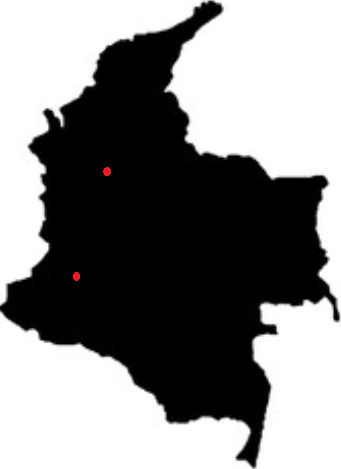
\includegraphics[scale=0.42]{img/colombia-logo.png}
	~
\end{aside}

\section{Educación}
\begin{entrylist}
	\entry
	{Aug. 20 - Hoy}
	{PhD en Ciencias de la Computación}
	{{
\includegraphics[scale=0.05]{img/unicauca-logo.png}} Universidad del Cauca, CO} 
	{Estudios de doctorado enfocados en la mejora y aseguramiento de calidad en el desarrollo de software utilizando Aproximaciones ágiles. Actualmente, realizando trabajo de investigación en la evaluación de modelos para DevOps soportado en técnicas de inferencia utilizando inteligencia artificial.}
	
	\entry
	{Aug. 20 - Hoy}
	{Maestría (MSc) en Computación}
	{ \raisebox{-1.5ex}{
\includegraphics[scale=0.05]{img/unicauca-logo.png} Universidad del Cauca, CO}}
	{Estudios de posgrado enfocados a la mejora de procesos y evaluación de DevOps en empresas desarrolladoras de software.}
	
	\entry
	{Aug. 18 - Hoy}
	{Pregrado de Astronomía}
	{ \raisebox{-1.5ex}{
\includegraphics[scale=0.05]{img/udea-logo.png}Universidad de Antioquia, CO}}
	{Actualmente estudiando la malla curricular para obtener el título de Astrónomo.}
	
	\entry
	{Aug. 11 - Mar. 17}
	{Pregrado de Ingeniería de Sistemas}
	{ \raisebox{-1.5ex}{
\includegraphics[scale=0.05]{img/unicauca-logo.png} Universidad del Cauca, CO}}
	{Profesional en ingeniería de sistemas con la habilidad de identificar y resolver problemas relacionados a la industria TI..

\href{https://drive.google.com/file/d/1G3Y7GhNoIpcnDgohF6aI6t12TZSkDqYa/view?usp=sharing}
{\raisebox{-0.35ex}{
\includegraphics[scale=0.025]{img/certificado-logo.png}}{\addfontfeature{Color=pblue}\ul{\textit{Ver certificado}}}}
    
\href{https://drive.google.com/file/d/1k7jfkqE6BgAO2oRgTTbBabDCLhrU8XFm/view?usp=sharing}{\raisebox{-0.35ex}{
\includegraphics[scale=0.011]{img/diploma-logo.png}}{\addfontfeature{Color=pblue}\ul{    \textit{Diploma}}}}
	}
	
	\entry
	{Jan. 04 - Dic. 10}
	{Bachiller Técnico en Desarrollo de Software}
	{ \raisebox{-1.5ex}{
\includegraphics[scale=0.007]{img/industrial-logo.png} Instituto Técnico Industrial, CO}}
	{Grado de bachiller con énfasis en desarrollo de software.}
	
	\entry
	{Jan. 00 - Dic. 04}
	{Grado en básica primaria.}
	{ \raisebox{-1.5ex}{
\includegraphics[scale=0.007]{img/industrial-logo.png} Instituto Técnico Industrial, CO}}
	{Grado en educación básica primaria}
\end{entrylist}

\section{Proyectos}
\begin{entrylist}
	\entry
	{Hoy}
	{APP PERSONAS BANCOLOMBIA}
	{ \raisebox{-1.5ex}{
\includegraphics[scale=0.05]{img/bancolombia-logo.png} Bancolombia, Medellín, CO}}
	{Trabajo como proveedor externo realizando tareas relacionadas a la implementación de servicios, canales de comunicación, plataforma, base de datos y BackEnd para las nuevas iniciativas en los proyectos de la organización.}
	
	\entry
	{Nov. 17}
	{AUDAMEDIC – AUDATEX México}
	{ \raisebox{-1.5ex}{
\includegraphics[scale=0.05]{img/sitis-logo.png} SITIS SAS, Popayán, CO}}
	{Desarrollo del sistema de aseguramiento para Audatex MX utilizando tecnología JAVA EE para BackEnd y Primefaces en FrontEnd.}
	  
	\entry
	{Sep. 15}
	{SMAC-JPA}
	{ \raisebox{-1.5ex}{DAWSIN SAS, Popayán, CO}}
	{Desarrollo del sistema de aseguramiento para la AIC-EPSI. Uso de tecnología JAVA EE con servicios REST/API para BackEndd y Angular 5 para FrontEnd.}
	
	\entry
	{Aug. 14}
	{CENSO WEB}
	{ \raisebox{-1.5ex}{DAWSIN SAS, Popayán, CO}}
	{Systema desarrollado en PGP para capturar la información del censo de la población indígena en el cabildo de Pitayó-Cauca.}
	
	\entry
	{Jan. 14}
	{VENTAS MOVIL}
	{ \raisebox{-1.5ex}{DAWSIN SAS, Popayán, CO}}
	{Sistema de ventas desarrollado en JAVA y Android nativo para su integración con la aplicación de ventas TAT.}
	
	\entry
	{May. 13}
	{NETCOM}
	{ \raisebox{-1.5ex}{DAWSIN SAS, Popayán, CO}}
	{Desarrolllo y validación de la arquitectura del proyecto utilizando modelos de consulta genéricos.}
	
\end{entrylist}

\section{Certificaciones}
\begin{entrylist}
	\entry
	{2020}
	{Desarrollo Ágil de software}
	{ \raisebox{-1.5ex}{
\includegraphics[scale=0.3]{img/linkedin-logo.png}}}
	{\href{https://drive.google.com/file/d/1Exu_C3WSs1GdBZsTsl7TQbTIOxiHJco7/view?usp=sharing}
{\raisebox{-0.35ex}{
\includegraphics[scale=0.025]{img/certificado-logo.png}}{\addfontfeature{Color=pblue}\ul{\textit{Ver certificado}}}}}
	
	\entry
	{2020}
	{Introduction to Astrophysics}
	{ \raisebox{-1.5ex}{
\includegraphics[scale=0.2]{img/edx-logo.png}}}
	{\href{https://drive.google.com/file/d/1wFflupPYMjYnNPa2viIrOeH5QaQjDQxa/view?usp=sharing}
{\raisebox{-0.35ex}{\includegraphics[scale=0.025]{img/certificado-logo.png}}{\addfontfeature{Color=pblue}\ul{\textit{Ver certificado}}}}}
	
	\entry
	{2020}
	{Java EE: Design Patterns and Architecture}
	{ \raisebox{-1.5ex}{\includegraphics[scale=0.3]{img/linkedin-logo.png}}}
	{\href{https://drive.google.com/file/d/1X8KAiItYbozqOugfP0LVEszACZAVvalk/view?usp=sharing}
{\raisebox{-0.35ex}{\includegraphics[scale=0.025]{img/certificado-logo.png}}{\addfontfeature{Color=pblue}\ul{\textit{Ver certificado}}}}}
	
	\entry
	{2020}
	{Java avanzado, buenas prácticas}
	{ \raisebox{-1.5ex}{\includegraphics[scale=0.3]{img/linkedin-logo.png}}}
	{\href{https://drive.google.com/file/d/1SglLIDQ8DfaV1yGeXNYxZIyvp8Kj6pio/view?usp=sharing}
{\raisebox{-0.35ex}{\includegraphics[scale=0.025]{img/certificado-logo.png}}{\addfontfeature{Color=pblue}\ul{\textit{Ver certificado}}}}}
	
	\entry
	{2020}
	{Python para data scientist avanzado}
	{ \raisebox{-1.5ex}{\includegraphics[scale=0.3]{img/linkedin-logo.png}}}
	{\href{https://drive.google.com/file/d/1ETa1PgGn3-FVyB6pXUBmGpTgyQKK_dZh/view?usp=sharing}
{\raisebox{-0.35ex}{\includegraphics[scale=0.025]{img/certificado-logo.png}}{\addfontfeature{Color=pblue}\ul{\textit{Ver certificado}}}}}
	
	\entry
	{2020}
	{Contribution to observation of near-Earth objects}
	{ \raisebox{-1.5ex}{\includegraphics[scale=0.07]{img/nasa-logo.png}}}
	{\href{https://drive.google.com/file/d/168wBuL1g379P9S0NWkMZUV6TKbQpATpM/view?usp=sharing}
{\raisebox{-0.35ex}{\includegraphics[scale=0.025]{img/certificado-logo.png}}{\addfontfeature{Color=pblue}\ul{\textit{Ver certificado}}}}}
	
	\entry
	{2019}
	{Security Core Training}
	{ \raisebox{-1.5ex}{\includegraphics[scale=0.05]{img/sans-logo.png}}}
	{\href{https://drive.google.com/file/d/17w7DkG3eSB_vX8RVpsKdzPut914wRJwE/view?usp=sharing}
{\raisebox{-0.35ex}{\includegraphics[scale=0.025]{img/certificado-logo.png}}{\addfontfeature{Color=pblue}\ul{\textit{Ver certificado}}}}}
	
	\entry
	{2016}
	{Scrum Fundamentals Certified Credential}
	{ \raisebox{-1.5ex}{\includegraphics[scale=0.035]{img/scrumstudy-logo.jpg}}}
	{\href{https://drive.google.com/file/d/1zEMOSdEmqP5sZ-oQow2gGgqcSKYNhvp6/view?usp=sharing}
{\raisebox{-0.35ex}{\includegraphics[scale=0.025]{img/certificado-logo.png}}{\addfontfeature{Color=pblue}\ul{\textit{Ver certificado}}}}}
	
\end{entrylist}

\section{Publicaciones y Conferencias}
\begin{entrylist}
	\entry
	{2020}
	{Progresconfig: Un proceso de GCS}
	{ \raisebox{-1.5ex}{\includegraphics[scale=0.15]{img/risti-logo.png}}}
	{Artículo aceptado en la Revista Ibérica de Sistemas y Tecnologías de la Información (RISTI). Ponente del artículo en: III Congreso Internacional de Sistemas Inteligentes y Nuevas Tecnologías: Tendencias Interdisciplinarias en Salud (COISINT 2020)
    
{\href{https://drive.google.com/file/d/1UAspvy3NgSpDMQh68TYh3A5M1i-WkCWU/view?usp=sharing}{\raisebox{-0.35ex}{\includegraphics[scale=0.025]{img/certificado-logo.png}}{\addfontfeature{Color=pblue}\ul{\textit{Ver certificado}}}}}
	}
	
	\entry
	{2020}
	{SCMOnto: Una ontología de GCS}
	{ \raisebox{-1.5ex}{\includegraphics[scale=0.15]{img/risti-logo.png}}}
	{Artículo aceptado en la Revista Ibérica de Sistemas y Tecnologías de la Información (RISTI). Ponente del artículo en: XV Jornadas Iberoamericanas de Ingeniería de Software e Ingeniería del Conocimiento (JIISIC 2020)
    
{\href{https://drive.google.com/file/d/1XFyQmaJYHnE0CFuQ2sXhUQwdl63ygry-/view?usp=sharing}{\raisebox{-0.35ex}{\includegraphics[scale=0.025]{img/certificado-logo.png}}{\addfontfeature{Color=pblue}\ul{\textit{Ver certificado}}}}}
	}
	
	\entry
	{2015}
	{II Jornada Iberoamericana de Interacción Humano Computador}
	{}
	{Asistente.
    
{\href{https://drive.google.com/file/d/1GhB6CtWBM6grahODRsxH6nRxh8daVpbH/view?usp=sharing}{\raisebox{-0.35ex}{\includegraphics[scale=0.025]{img/certificado-logo.png}}{\addfontfeature{Color=pblue}\ul{\textit{Ver certificado}}}}}
	}
\end{entrylist}

\newpage

\section{Experiencia de Voluntariado}
\begin{entrylist}
	  
	\entry
	{Jul. 18 - Hoy}
	{Monitor}
	{{\includegraphics[scale=0.05]{img/udea-logo.png}} Universidad de Antioquia, CO} 
	{Asistir y guiar a estudiantes de primeros semestre en áreas relacionadas a las ciencias exactas en conceptos y funcamentos de algoritmia y programación orientada a objetos.}
	  
	\entry
	{Sep. 18 - Mar. 20}
	{Codirector de Trabajo de Grado}
	{{\includegraphics[scale=0.05]{img/unicauca-logo.png}} Universidad del Cauca, CO} 
	{Soportar y hacer seguimiento a proyectos de trabajo de grado de estudiantes de ingeniería de sistemas en la Universidad del Cauca.}
	
	\entry
	{Aug. 15 - Dec 17}
	{Monitor}
	{{\includegraphics[scale=0.05]{img/unicauca-logo.png}} Universidad del Cauca, CO} 
	{Asistir a estudiantes de semestres inferiores en aspectos relacionados al desarrollo de aplicaciones web usando arquitecturas empresariales, aplicación de mejores prácticas para el desarrollo de software y guía en procesos como: integración continua, documentación de código, pruebas unitarias, patrones de diseño y mejores prácticas para el desarrollo orientado a objetos.}
	
\end{entrylist}


\section{Referencias}
\begin{entrylist}
	  
	\entry
	{Académico}
	{PhD. MSc. Eng. César Pardo}
	{Ingeniero de Sistemas} 
	{Contacto: +573508479834, Popayán, CO.}
	
	\entry
	{Académico}
	{PhD. MSc. Eng. Fracisco Pino}
	{Ingeniero de Sistemas} 
	{Contacto: +573218942563, Popayán, CO.}
	
	\entry
	{Laboral}
	{Eng. Jorge Gomez}
	{Ingeniero de Sistemas} 
	{Contacto: +573153564186, Popayán, CO.}
	
	\entry
	{Laboral}
	{Lic. Felipe Salazar}
	{Administrador de empresas} 
	{Contacto: +573136066832, Cali, CO.}
	
	\entry
	{Personal}
	{Eng. Edward Orozco}
	{Ingeniero de Sistemas} 
	{Contacto: +573174281839, Popayán, CO.}
	
	\entry
	{Personal}
	{Lic. Rocio Orozco}
	{Maestra en Artes Plásticas} 
	{Contacto: +3156215575, Cali, CO.}
	
\end{entrylist}


\vspace{0.5cm}
\begin{center}
	\emph{Para todos los efectos legales certifico que todas las respuestas e informaciones anotadas por mí, en la presente hoja de vida son veraces (C.S.T.Art.62 num. 1st)}
\end{center}

\begin{flushright}
    	\emph{{\includegraphics[scale=0.55]{img/firma.JPG}}}
\end{flushright}
\begin{flushright}
	\emph{\textbf{CARLOS EDUARDO OROZCO GARCÉS}}
\end{flushright}
\begin{flushright}
	\emph{C.C. 1061772393. Popayán, CO}
\end{flushright}

\end{document}
